\documentclass{beamer}
\mode<presentation>{
  \usetheme{Boadilla}
  \usefonttheme[onlylarge]{structurebold}
  \usefonttheme[stillsansseriflarge]{serif}
  \setbeamerfont*{frametitle}{size=\normalsize,series=\bfseries}
  % \setbeamertemplate{navigation symbols}{}
  \setbeamercovered{transparent}
}
\usepackage[english]{babel}
\usepackage[latin1]{inputenc}
\usepackage{times}
\usepackage[T1]{fontenc}
\usepackage{amsmath}
\usepackage{amssymb}
\usepackage{esint}
\usepackage{hyperref}
\usepackage{tikz}
\usepackage{xkeyval}
\usepackage{xargs}
\usepackage{verbatim}
\usepackage{listings}
\usepackage{multimedia}
\usepackage{bm}
\usepackage{siunitx}
\usetikzlibrary{
  arrows,
  calc,
  decorations.pathmorphing,
  decorations.pathreplacing,
  decorations.markings,
  fadings,
  positioning,
  shapes,
  arrows.meta
}
\usepgfmodule{oo}

\pgfdeclareradialshading{glow2}{\pgfpoint{0cm}{0cm}}{
  color(0mm)=(white);
  color(2mm)=(white);
  color(8mm)=(black);
  color(10mm)=(black)
}
\pgfdeclareradialshading{glow}{\pgfpoint{0cm}{0cm}}{
  color(0mm)=(white);
  color(5mm)=(white);
  color(9mm)=(black);
  color(10mm)=(black)
}

\begin{tikzfadingfrompicture}[name=glow fading]
  \shade [shading=glow] (0,0) circle (1);
\end{tikzfadingfrompicture}

\begin{tikzfadingfrompicture}[name=glow2 fading]
  \shade [shading=glow2] (0,0) circle (1);
\end{tikzfadingfrompicture}

\mode<handout>{
  \usepackage{pgfpages}
  \pgfpagesuselayout{4 on 1}[a4paper,landscape,border shrink=5mm]
  \setbeamercolor{background canvas}{bg=black!10}
}

\newcommand\pgfmathsinandcos[3]{%
  \pgfmathsetmacro#1{sin(#3)}%
  \pgfmathsetmacro#2{cos(#3)}%
}
\newcommand\LongitudePlane[3][current plane]{%
  \pgfmathsinandcos\sinEl\cosEl{#2} % elevation
  \pgfmathsinandcos\sint\cost{#3} % azimuth
  \tikzset{#1/.estyle={cm={\cost,\sint*\sinEl,0,\cosEl,(0,0)}}}
}
\newcommand\LatitudePlane[3][current plane]{%
  \pgfmathsinandcos\sinEl\cosEl{#2} % elevation
  \pgfmathsinandcos\sint\cost{#3} % latitude
  \pgfmathsetmacro\yshift{\cosEl*\sint}
  \tikzset{#1/.estyle={cm={\cost,0,0,\cost*\sinEl,(0,\yshift)}}} %
}
\newcommand\DrawLongitudeCircle[2][1]{
  \LongitudePlane{\angEl}{#2}
  \tikzset{current plane/.prefix style={scale=#1}}
  % angle of "visibility"
  \pgfmathsetmacro\angVis{atan(sin(#2)*cos(\angEl)/sin(\angEl))} %
  \draw[current plane] (\angVis:1) arc (\angVis:\angVis+180:1);
  \draw[current plane,dashed] (\angVis-180:1) arc (\angVis-180:\angVis:1);
}
\newcommand\DrawLatitudeCircleArrow[2][1]{
  \LatitudePlane{\angEl}{#2}
  \tikzset{current plane/.prefix style={scale=#1}}
  \pgfmathsetmacro\sinVis{sin(#2)/cos(#2)*sin(\angEl)/cos(\angEl)}
  % angle of "visibility"
  \pgfmathsetmacro\angVis{asin(min(1,max(\sinVis,-1)))}
  \draw[current plane,decoration={markings, mark=at position 0.6 with {\arrow{<}}},postaction={decorate},line width=.6mm] (\angVis:1) arc (\angVis:-\angVis-180:1);
  \draw[current plane,dashed,line width=.6mm] (180-\angVis:1) arc (180-\angVis:\angVis:1);
}
\newcommand\DrawLatitudeCircle[2][1]{
  \LatitudePlane{\angEl}{#2}
  \tikzset{current plane/.prefix style={scale=#1}}
  \pgfmathsetmacro\sinVis{sin(#2)/cos(#2)*sin(\angEl)/cos(\angEl)}
  % angle of "visibility"
  \pgfmathsetmacro\angVis{asin(min(1,max(\sinVis,-1)))}
  \draw[current plane] (\angVis:1) arc (\angVis:-\angVis-180:1);
  \draw[current plane,dashed] (180-\angVis:1) arc (180-\angVis:\angVis:1);
}
\newcommand\coil[1]{
  {\rh * cos(\t * pi r)}, {\apart * (2 * #1 + \t) + \rv * sin(\t * pi r)}
}
\makeatletter
\define@key{DrawFromCenter}{style}[{->}]{
  \tikzset{DrawFromCenterPlane/.style={#1}}
}
\define@key{DrawFromCenter}{r}[1]{
  \def\@R{#1}
}
\define@key{DrawFromCenter}{center}[(0, 0)]{
  \def\@Center{#1}
}
\define@key{DrawFromCenter}{theta}[0]{
  \def\@Theta{#1}
}
\define@key{DrawFromCenter}{phi}[0]{
  \def\@Phi{#1}
}
\presetkeys{DrawFromCenter}{style, r, center, theta, phi}{}
\newcommand*\DrawFromCenter[1][]{
  \setkeys{DrawFromCenter}{#1}{
    \pgfmathsinandcos\sint\cost{\@Theta}
    \pgfmathsinandcos\sinp\cosp{\@Phi}
    \pgfmathsinandcos\sinA\cosA{\angEl}
    \pgfmathsetmacro\DX{\@R*\cost*\cosp}
    \pgfmathsetmacro\DY{\@R*(\cost*\sinp*\sinA+\sint*\cosA)}
    \draw[DrawFromCenterPlane] \@Center -- ++(\DX, \DY);
  }
}
\newcommand*\DrawFromCenterText[2][]{
  \setkeys{DrawFromCenter}{#1}{
    \pgfmathsinandcos\sint\cost{\@Theta}
    \pgfmathsinandcos\sinp\cosp{\@Phi}
    \pgfmathsinandcos\sinA\cosA{\angEl}
    \pgfmathsetmacro\DX{\@R*\cost*\cosp}
    \pgfmathsetmacro\DY{\@R*(\cost*\sinp*\sinA+\sint*\cosA)}
    \draw[DrawFromCenterPlane] \@Center -- ++(\DX, \DY) node {#2};
  }
}
\makeatother

% not mandatory, but I though it was better to set it blank
\setbeamertemplate{headline}{}
\def\beamer@entrycode{\vspace{-\headheight}}

\tikzstyle{snakearrow} = [decorate, decoration={pre length=0.2cm,
  post length=0.2cm, snake, amplitude=.4mm,
  segment length=2mm},thick, ->]

%% document-wide tikz options and styles

\tikzset{%
  % >=latex, % option for nice arrows
  inner sep=0pt,%
  outer sep=2pt,%
  mark coordinate/.style={inner sep=0pt,outer sep=0pt,minimum size=3pt,
    fill=black,circle}%
}
\tikzset{
  % Define standard arrow tip
  >=stealth',
  % Define style for boxes
  punkt/.style={
    rectangle,
    rounded corners,
    draw=black, very thick,
    text width=8em,
    minimum height=2.5em,
    text centered},
}

\tikzset{onslide/.code args={<#1>#2}{%
    \only<#1>{\pgfkeysalso{#2}}
    % \pgfkeysalso doesn't change the path
  }}
\tikzset{alt/.code args={<#1>#2#3}{%
    \alt<#1>{\pgfkeysalso{#2}}{\pgfkeysalso{#3}}
    % \pgfkeysalso doesn't change the path
  }}
\tikzset{temporal/.code args={<#1>#2#3#4}{%
    \temporal<#1>{\pgfkeysalso{#2}}{\pgfkeysalso{#3}}{\pgfkeysalso{#4}}
    % \pgfkeysalso doesn't change the path
  }}

\makeatletter
\newbox\@backgroundblock
\newenvironment{backgroundblock}[2]{%
  \global\setbox\@backgroundblock=\vbox\bgroup%
  \unvbox\@backgroundblock%
  \vbox to0pt\bgroup\vskip#2\hbox to0pt\bgroup\hskip#1\relax%
}{\egroup\egroup\egroup}
\addtobeamertemplate{background}{\box\@backgroundblock}{}
\makeatother

% \def\timeleft{15:00->14:55}

\title{NaCs lab update}
\date{April 06, 2018}
\author{Yichao Yu}
\institute{Ni Group}

\begin{document}

\pgfdeclarelayer{tweezer}
\pgfsetlayers{tweezer,main}
\pgfooclass{tweezer}{
  \method tweezer() {
  }
  \method drawTweezer(#1,#2,#3) {
    \begin{pgfonlayer}{tweezer}
      \shade[shading=radial,path fading=glow fading,shift={(#1,#2)},rotate=90,yscale=1,
      fill opacity=0.9,inner color=#3]
      plot[draw,samples=200,domain=-1.5:1.5] function {sqrt(0.01 + x**2 / 5)}
      -- plot[draw,samples=200,domain=1.5:-1.5] function {-sqrt(0.01 + x**2 / 5)};
    \end{pgfonlayer}
  }
  \method drawAtom(#1,#2,#3,#4) {
    \fill [#4,path fading=glow2 fading] (#1,#2) circle (#3);
  }
  \method drawNaAtom(#1,#2,#3) {
    \pgfoothis.drawAtom(#1,#2,#3,orange);
  }
  \method drawCsAtom(#1,#2,#3) {
    \pgfoothis.drawAtom(#1,#2,#3,blue);
  }
  \method drawNaTweezer(#1,#2) {
    \pgfoothis.drawTweezer(#1,#2,orange!35!black!30);
  }
  \method drawCsTweezer(#1,#2) {
    \pgfoothis.drawTweezer(#1,#2,blue!30!black!30);
  }
  \method up(#1,#2) {
    \pgfoothis.drawCsTweezer(#1,#2);
    \pgfoothis.drawNaAtom(#1,#2+0.06,0.12);
    \pgfoothis.drawCsAtom(#1,#2-0.06,0.16);
  }
  \method down(#1,#2) {
    \pgfoothis.drawCsTweezer(#1,#2);
    \pgfoothis.drawCsAtom(#1,#2+0.06,0.16);
    \pgfoothis.drawNaAtom(#1,#2-0.06,0.12);
  }
  \method naTrap(#1,#2) {
    \pgfoothis.drawNaTweezer(#1,#2);
    \pgfoothis.drawNaAtom(#1,#2,0.12);
  }
  \method csTrap(#1,#2) {
    \pgfoothis.drawCsTweezer(#1,#2);
    \pgfoothis.drawCsAtom(#1,#2,0.16);
  }
}
\pgfoonew \mytweezer=new tweezer()

{
  \usebackgroundtemplate{
    \makebox[\paperwidth][c]{\centering\includegraphics[width=\paperwidth]{front_bg.png}}
  }
  \setbeamercolor{title}{fg=cyan!50}
  \setbeamercolor{author}{fg=white}
  \setbeamercolor{institute}{fg=white}
  \setbeamercolor{date}{fg=white}
  \begin{frame}{}
    \titlepage
  \end{frame}
}

\begin{frame}{Photoassociation/EIT}
  \begin{center}
    \begin{tikzpicture}
      \node at (0, 0) {\includegraphics[width=8cm]{pa.png}};
      \node[below] at (0, -1.1) {\small PA detuning (GHz)};
      \visible<2-3>{
        \node at (-3, -4) {\includegraphics[width=5cm]{pa_linewidth.png}};
      }
      \visible<4->{
        \node at (-3, -4) {\includegraphics[width=5cm]{eit.png}};
      }
      \visible<3->{
        \begin{scope}[shift={(0.5, -6)},scale=0.55]
          \draw[->,line width=1.2] (0, 0) -- (0, 8);
          \node[above,rotate=90] at (0, 4) {\small Energy};
          \draw[->,line width=1.2] (0, 0) -- (8, 0);
          \node[below] at (4, 0) {\small Internuclear distance};

          \draw[cyan!85!blue] (1.0269 + 0.25, 2.5) -- (7.25, 2.5);
          \only<2->{
            \draw[cyan!85!blue] (1.0793 + 0.25, -0.4631 + 2.5) -- (4.5 + 0.25, -0.4631 + 2.5);
          }

          \draw[red] (1.1102 - 0.75, -0.7720 + 7.5) -- (6 - 0.75, -0.7720 + 7.5);
          \draw[red] (1.1576 - 0.75, -1.0595 + 7.5) -- (4.5 - 0.75, -1.0595 + 7.5);

          \draw[line width=1.1,cyan!85!blue]
          plot[samples=200,domain=1:7,variable=\x]
          ({\x + 0.25}, {6.8*\x^(-3.4)-6.5*\x^(-1.7) + 2.5});
          \node[cyan!85!blue] at (3.75, 1.0) {$a^3\Sigma^+$};

          \draw[line width=1.1,red]
          plot[samples=200,domain=1:7.5,variable=\x]
          ({\x - 0.75}, {9.2*\x^(-2.5)-9.0*\x^(-1.3) + 7.5});
          \node[above right,red] at (0.55, 7.2) {$c^3\Sigma^+$};

          \mytweezer.drawNaAtom(6.55, 2.6, 0.12)
          \mytweezer.drawCsAtom(7.05, 2.6, 0.10)

          \only<2->{
            \mytweezer.drawNaAtom(4.08, 2.15, 0.12)
            \mytweezer.drawCsAtom(4.25, 2.15, 0.10)
          }

          \draw[->,blue!50!orange,line width=0.8] (6.8, 2.7) -- (4.5 - 0.75, -0.85 + 7.5);
          \only<2->{
            \draw[->,green!80!black,line width=0.8] (4.165, 2.25) -- (4.45 - 0.75, -0.85 + 7.5);
          }
        \end{scope}
      }
    \end{tikzpicture}
  \end{center}
\end{frame}

\begin{frame}{Getting to ground electronic state}
  \begin{center}
    \begin{columns}
      \column{6.5cm}
      \begin{tikzpicture}
        \begin{scope}[scale=0.7]
          \draw[->,line width=1.2] (0, 0) -- (0, 8);
          \node[above,rotate=90] at (0, 4) {Energy};
          \draw[->,line width=1.2] (0, 0) -- (8, 0);
          \node[below] at (4, -0.5) {Internuclear distance};

          \draw[cyan!85!blue] (1.0269 + 0.25, 2.5) -- (7.25, 2.5);
          \draw[cyan!85!blue] (1.0793 + 0.25, -0.4631 + 2.5) -- (4.5 + 0.25, -0.4631 + 2.5);

          \draw[line width=1.1,cyan!85!blue]
          plot[samples=200,domain=1:7,variable=\x]
          ({\x + 0.25}, {6.8*\x^(-3.4)-6.5*\x^(-1.7) + 2.5});
          \node[cyan!85!blue] at (3.75, 1.0) {$a^3\Sigma^+$};

          \draw[line width=1.1,red]
          plot[samples=200,domain=1:7.5,variable=\x]
          ({\x - 0.75}, {9.2*\x^(-2.5)-9.0*\x^(-1.3) + 7.5});
          \node[above right,red] at (0.55, 7.2) {$c^3\Sigma^+$};

          \mytweezer.drawNaAtom(6.55, 2.6, 0.12)
          \mytweezer.drawCsAtom(7.05, 2.6, 0.10)

          \mytweezer.drawNaAtom(4.08, 2.15, 0.12)
          \mytweezer.drawCsAtom(4.25, 2.15, 0.10)

          \draw[black!40,dashed,line width=1] (0.25, 5) -- (7.25, 5);

          \draw[->,green!80!black,line width=0.8] (6.8, 2.7) -- (5.5, 5)
          node[midway, right] {$\approx1038nm$};
          \draw[->,green!80!black,line width=0.8] (5.45, 5) -- (4.165, 2.25);
        \end{scope}
      \end{tikzpicture}
      \column{4cm}
      \begin{block}{}
        \begin{itemize}
        \item<2-> New laser
        \item<3-> New beam path
        \item<4-> PA on deeply bound state
        \item<5-> Lesson about mirror mount
        \end{itemize}
      \end{block}
    \end{columns}
  \end{center}
\end{frame}

\begin{frame}{Cooling multiple atoms}
  \begin{center}
    \begin{tikzpicture}
      \visible<1>{
        \node[align=center] at (0, 0) {\includegraphics[width=6cm]{cs_diff_trapf.png}\\
          Very different sideband frequencies
        };
      }
      \visible<2>{
        \node[align=center] at (0, 0) {
          Align trap frequencies\\
          \includegraphics[width=9cm]{cs_trapf.png}
        };
      }
      \visible<3-4>{
        \node[align=center] at (0, 0) {
          \includegraphics[width=6cm]{cs_same_trapf.png}\\
          Overall shift on both carrier and sideband.
        };
      }
      \visible<4>{
        \fill[white,opacity=0.85] (-5, -4) rectangle (5, 4);
        \node[align=center,text width=6cm] at (0, 0) {
          {\Large Possible causes??}\\\vspace{0.3cm}
          \begin{itemize}
          \item Trap light shift
          \item Raman beam light shift
          \item Magnetic field difference
          \item $\cdots$
          \end{itemize}
        };
      }
    \end{tikzpicture}
  \end{center}
\end{frame}

\begin{frame}{Alignment between tweezer polarization and B field}
  \begin{center}
    \begin{tikzpicture}
      \begin{scope}[shift={(-0.75, 0)},onslide=<3->{rotate=-6}]
        \mytweezer.drawCsTweezer(0, 0);
        \visible<2->{
          \draw[blue,->,line width=1] (0, 0.5) -- (0, -0.5) node[below] {\tiny $B_{eff}$};
        }
      \end{scope}
      \begin{scope}[shift={(0.75, 0)},onslide=<3->{rotate=6}]
        \mytweezer.drawCsTweezer(0, 0);
        \visible<2->{
          \draw[blue,->,line width=1] (0, 0.5) -- (0, -0.5) node[below] {\tiny $B_{eff}$};
        }
      \end{scope}
      \draw[red,->,line width=1.5] (-1.2, -2) -- (1.2, -2) node[right] {$B_{bias}$};
      \visible<-4>{
        \node[text width=6cm,align=center] at (5.5, 0) {
          \begin{block}{}
            \begin{itemize}
            \item<2-> Tweezer circular polarization
            \item<3-> Tweezer rotation
            \end{itemize}
          \end{block}
          {
            \visible<4>{
              \begin{block}{Sensitive to ...}
                \begin{itemize}
                \item Tweezer polarization
                \item Tweezer alignment
                \item B field direction
                \item Hyperfine state
                \end{itemize}
              \end{block}
            }
          }
        };
      }
      \visible<5->{
        \node[red] at (7.5, 3.55) {$\Delta B_y=0.0G$};
        \node at (5.5, 1.9) {\includegraphics[width=6.5cm]{../../experiments/cs_coprop_201712/imgs/data_20171228_resonance_mf4.pdf}};
        \node[red] at (7.5, -0.25) {$\Delta B_y=0.5G$};
        \node at (5.5, -1.9) {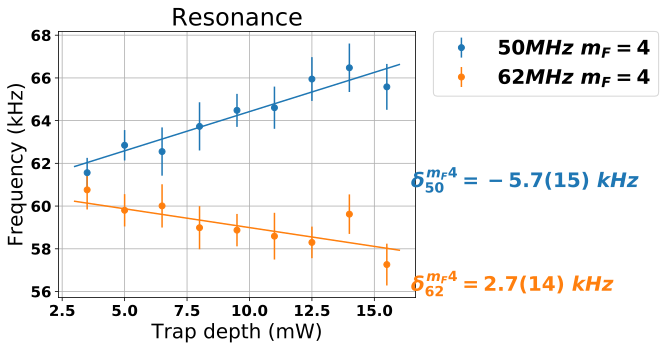
\includegraphics[width=6.5cm]{../../experiments/cs_coprop_201712/imgs/data_20180103_resonance_mf4.pdf}};
      }
      \visible<6->{
        \fill[white,opacity=0.9] (-2, -3.55) rectangle (8.75, 3.8);
        \node[text width=8cm,align=center,right] at (0, 0) {
          \begin{itemize}
          \item Trap polarization\\
            $C=0.0545(94)$\\
            or $0.30(10) \%$ power in wrong polarization
          \item Angle between tweezers\\
            $1.10(58)^\circ$\\
            or $0.30(16)$mm shift on Fourier plane.
          \end{itemize}
        };
      }
    \end{tikzpicture}
  \end{center}
\end{frame}

\end{document}
